% Title: gl2ps_renderer figure
% Creator: GL2PS 1.4.0, (C) 1999-2017 C. Geuzaine
% For: Octave
% CreationDate: Tue Oct 26 18:57:12 2021
\setlength{\unitlength}{1pt}
\begin{picture}(0,0)
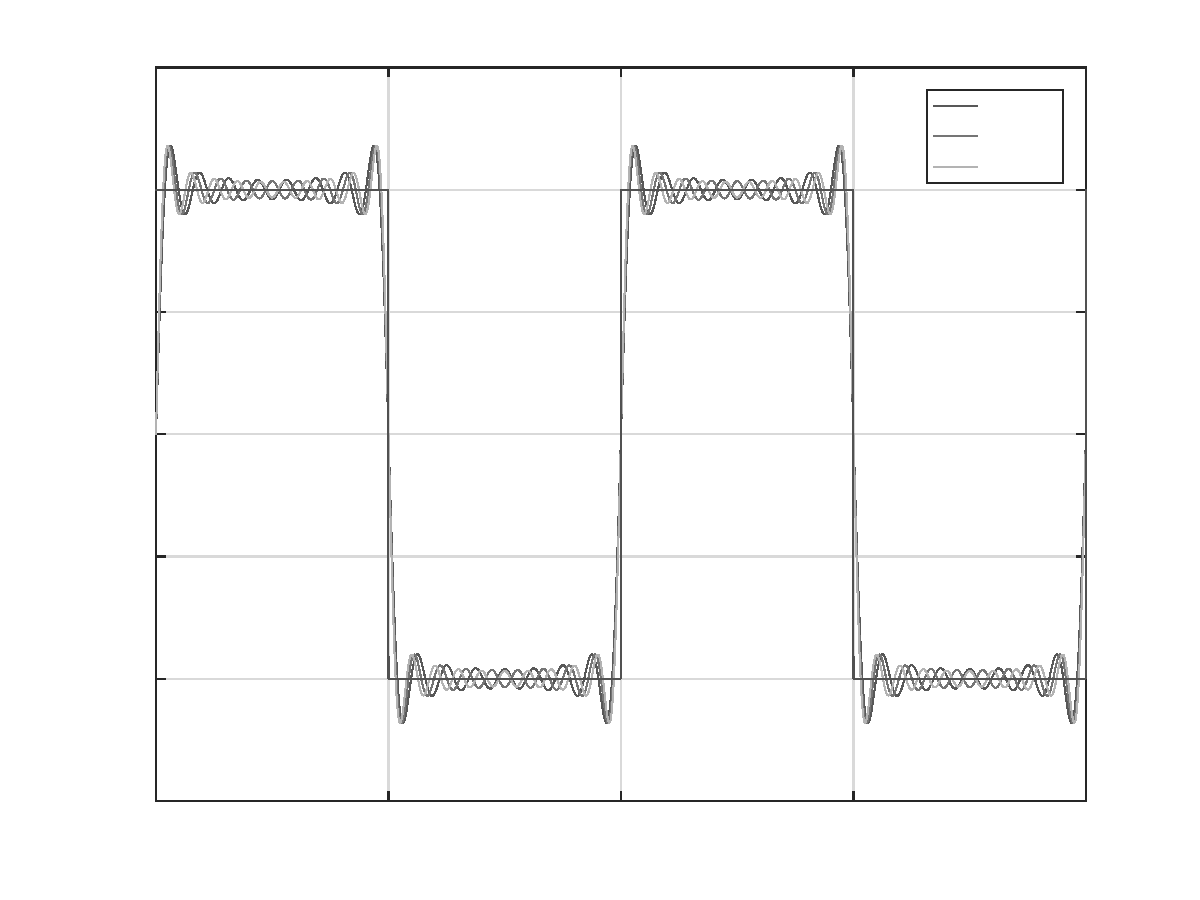
\includegraphics{figures/chap12/OUT/SquareWaveGray-inc}
\end{picture}%
\begin{picture}(576,432)(0,0)
\fontsize{10}{0}
\selectfont\put(74.88,40.0183){\makebox(0,0)[t]{\textcolor[rgb]{0.15,0.15,0.15}{{0}}}}
\fontsize{10}{0}
\selectfont\put(186.48,40.0183){\makebox(0,0)[t]{\textcolor[rgb]{0.15,0.15,0.15}{{0.5}}}}
\fontsize{10}{0}
\selectfont\put(298.08,40.0183){\makebox(0,0)[t]{\textcolor[rgb]{0.15,0.15,0.15}{{1}}}}
\fontsize{10}{0}
\selectfont\put(409.68,40.0183){\makebox(0,0)[t]{\textcolor[rgb]{0.15,0.15,0.15}{{1.5}}}}
\fontsize{10}{0}
\selectfont\put(521.28,40.0183){\makebox(0,0)[t]{\textcolor[rgb]{0.15,0.15,0.15}{{2}}}}
\fontsize{10}{0}
\selectfont\put(69.8755,47.52){\makebox(0,0)[r]{\textcolor[rgb]{0.15,0.15,0.15}{{-1.5}}}}
\fontsize{10}{0}
\selectfont\put(69.8755,106.2){\makebox(0,0)[r]{\textcolor[rgb]{0.15,0.15,0.15}{{-1}}}}
\fontsize{10}{0}
\selectfont\put(69.8755,164.88){\makebox(0,0)[r]{\textcolor[rgb]{0.15,0.15,0.15}{{-0.5}}}}
\fontsize{10}{0}
\selectfont\put(69.8755,223.56){\makebox(0,0)[r]{\textcolor[rgb]{0.15,0.15,0.15}{{0}}}}
\fontsize{10}{0}
\selectfont\put(69.8755,282.24){\makebox(0,0)[r]{\textcolor[rgb]{0.15,0.15,0.15}{{0.5}}}}
\fontsize{10}{0}
\selectfont\put(69.8755,340.92){\makebox(0,0)[r]{\textcolor[rgb]{0.15,0.15,0.15}{{1}}}}
\fontsize{10}{0}
\selectfont\put(69.8755,399.6){\makebox(0,0)[r]{\textcolor[rgb]{0.15,0.15,0.15}{{1.5}}}}
\fontsize{11}{0}
\selectfont\put(298.08,27.0183){\makebox(0,0)[t]{\textcolor[rgb]{0.15,0.15,0.15}{{$x$}}}}
\fontsize{11}{0}
\selectfont\put(46.8755,223.56){\rotatebox{90}{\makebox(0,0)[b]{\textcolor[rgb]{0.15,0.15,0.15}{{$\mathcal{S}_n[f](x)$}}}}}
\fontsize{11}{0}
\selectfont\put(298.08,409.6){\makebox(0,0)[b]{\textcolor[rgb]{0,0,0}{{Fourier Approximations of a Square Wave}}}}
\fontsize{9}{0}
\selectfont\put(472.118,381.239){\makebox(0,0)[l]{\textcolor[rgb]{0,0,0}{{$n = 15$}}}}
\fontsize{9}{0}
\selectfont\put(472.118,366.489){\makebox(0,0)[l]{\textcolor[rgb]{0,0,0}{{$n = 17$}}}}
\fontsize{9}{0}
\selectfont\put(472.118,351.739){\makebox(0,0)[l]{\textcolor[rgb]{0,0,0}{{$n = 19$}}}}
\end{picture}
